\section{Experiments}
\label{sec:experiments}
We compare the ExtRA framework with 
multiple strong baselines on extracting aspect terms from user reviews. 
We first introduce the dataset and the competing models, then
show the quantitative evaluation as well as qualitative analysis for
different models.

\subsection{Dataset}
\label{sec:dataset}
We use the customer review corpora of 6 kinds of product and service
\footnote{The data is available from
\url{http://times.cs.uiuc.edu/~wang296/Data/} and 
\url{https://www.yelp.com/dataset}} collected from popular websites, 
including Amazon, TripAdvisor and Yelp. 
The number of hotel reviews \cite{Wang2011LearningOD} in the original
corpus is huge. 
Therefore, we randomly sample 20\% of the reviews to perform our experiments.
The statistics of the corpora are shown in~\tabref{table:dataset}.

\begin{table}[th!]
\small
\centering
\vspace{-0.3cm}
\caption{Dataset statistics.} 
\label{table:dataset}
\vspace{-0.2cm}
\begin{tabular}{|c|c|c|}
\hline
\textbf{Product type} & \textbf{Source} & \textbf{\#Reviews} \\ \hline \hline
hotel        & TripAdvisor & 3,155,765   \\\hline
mobile phone & Amazon & 185,980  \\\hline
mp3 player   & Amazon & 30,996   \\\hline
laptop       & Amazon & 40,744   \\\hline
cameras & Amazon & 471,113  \\\hline
restaurant   & Yelp & 269,000   \\\hline
\end{tabular}
\vspace{-0.2cm}
\end{table}

%\label{sec:evaldataset}
Existing published aspect extraction datasets ~\cite{hu2004mining,popescu2007extracting,pavlopoulos2014aspect,ding2008holistic} 
include only fine-grained aspects from reviews,
which are not suitable for evaluating the performance of 
prominent aspects extraction. 
Therefore, we build a new evaluation dataset particularly 
for this task.
%\KZ{We need to explain why the data set is for 5 aspect only, not 10, 15?}
Following the previous work 
%Ganu et al
 ~\cite{ganu2009beyond,brody2010unsupervised,zhao2010jointly,wang2015sentiment} as well as
the popular commercial websites (e.g. TripAdvisor), 
which most manually labeled 3-6 prominent aspects for
rating, we set $K$ as five.
Therefore,  
we ask each annotator who are familiar with the domain 
to give 5 aspect terms which they think are most important
for each category. We have five annotators in total.
%In total, there are 25 aspect terms
%for each product type (including duplicates).
%Our annotated ground truths are all words by design, 
%since our baseline models can only extract aspect words.
%For example, the one set of annotations for hotel is 
%{\em room, price, location, service, utility}, and the annotations
%for restaurant is
%{\em location, price, food, service, cleanness}. 
%\footnote{The 
%	complete labeled set of ExtRA are released at \url{https://www.dropbox.com/s/dh20nvcziqf67j0/eval-dataset.txt?dl=0}.
%	Source code and processed data will be released after the review period.}
\footnote{The 
	complete labeled set of ExtRA is released at \url{https://adapt.seiee.sjtu.edu.cn/extra/}.
%	Source code and processed data will be released after the review period.
}
One prominent aspect can be expressed by different terms.
Thus, it is difficult to achieve a satisfied inner-agreement.
We propose two evaluation methods, especially the 
soft accuracy in \secref{sec:quaneval} to compensate this problem.
To acquire a relatively higher inner-agreement, 
we educate the annotators with top 100 frequent aspect candidates
as hints. Though, they are not required to pick up labels from 
the candidates.
The inter-annotator agreement of each
product type shown in \tabref{agreement} is computed as the average jaccard similarity between every two annotators.


%\begin{table}[th]
%	\small
%	\centering
%	\caption{Selected ground-truth labels.}
%	\label{table:labels}
%	\begin{tabular}{|c|l|}
%		\hline
%	Product type & Prominent aspects \\ \hline\hline
%		hotel
%		%			& price location room service bath staff \\\hline 
%		& room price location service utility \\ \hline
%		
%		camera
%		%			& battery image lens price appearance storage focus design mode memory carry operation \\\hline
%		& image lens battery memory carry \\ \hline
%		
%		restaurant
%		%			& food price location service environment cleans \\\hline
%		& location price food service cleanness \\ \hline
%	\end{tabular}
%\end{table}


%We aim to extract $K$ prominent aspects from review texts
%which are most important and representative
%for the given kind of products or services. 

\subsection{Baselines and ExtRA}
\label{sec:base}
We introduce three topic modeling based baselines for the task.
These are \textbf{LDA}~\cite{Blei2003LatentDA}, 
\textbf{BTM}~\cite{cheng2014btm} and  
\textbf{MG-LDA}~\cite{titov2008modeling}. MG-LDA is a strong
baseline which attempts to capture multi-grain topics (i.e. global \& local), where the local topics correspond to the rateable prominent aspects.
We treat each review as a document and perform those models
to extract $K$ topics.
% Each topic is expected to model an 
%prominent aspect for the given product or service.
Then, we select most probable words in 
each topic as our extracted aspect terms. 
To prevent extracting the same aspects ($w$) from different topics, 
we only keep $w$ for the topic $t$ with the highest 
probability $p(w|t)$ value, then re-select aspects for the other 
topics until we get $K$ different aspects. 
For fair comparison among different models, the number of 
target aspects $K$ is set as 5. The hyper-parameter of 
MG-LDA (global topics) is set to 30 with fine-tuning.

Another syntactic rule-based baseline model 
\textbf{AmodExt} is from the first stage of our framework. 
After extracting the aspect candidates using
\emph{amod-rule} in \secref{sec:candidate}, 
we sort the aspect candidates by 
their counts of extracted occurrences. 
Then select the top $K$ 
candidates as the prominent aspects.

\textbf{ABAE}~\cite{DBLP:conf/acl/HeLND17}  is a neural based model that can
to infer $K$ aspect types. 
Each \emph{aspect type} is a ranked list of representative words.
To generate $K$ prominent aspects, 
we first infer $K$ aspect types using \emph{ABAE}, 
then select the most representative word from each
aspect type. 
%We evaluate our framework as well as 
%the above baselines on the evaluation dataset.

%\paragraph{ExtRA Settings}
%\label{ourmodels}
For \textbf{ExtRA}, in the taxonomy construction stage, 
we use a two-stage K-means clustering method for synset matching task, 
and the cluster number
is auto-tuned using silhouette score~\cite{rousseeuw1987silhouettes}.
We use SkipGram~\cite{miko} model to train the embeddings
on review texts for k-means clustering. 
We set the dimension of the embeddings as 100
and run 64 epochs for each product corpora. 
In the aspect ranking stage, 
we empirically set the teleport probability $\alpha$
as $0.5$ which indicates that the expected walk-length
from the seeds is $\frac{1}{\alpha}=2$.
%The comparison of quantitative results are shown in \tabref{table:comparison}.}

\section{Experimental Results}
\label{sec:eval}
In this section, we first present the data set, 
then compare the fuzzy match results
of the ODL system with three other competing methods, before evaluating the
effects of incremental manual correction strategies.

\subsection{Dataset and Preprocessing}
%\JY{
%The dataset that we used for evaluation comes from real life ECG reports. 
%These reports come from different hospitals recorded at different times
%and they can be divided into many different formats. 
%For our experiment, we choose four different formats. 
%The examples about these formats are shown in \figref{fig:dataset}.
%One of the reason that we choose images in these four formats is 
%these four formats have the largest number of images. 
%Another reason is they contain different attributes, languages, and so on.
%}
The dataset we use are from real ECG reports, and are recorded at 
different times and different hospitals. Those reports can be 
divided into several different categories. We chose four typical kinds 
of reports which include many images and contain much useful information 
such as attributes, languages so that we could extract more data 
from them (see \figref{fig:dataset}).
% and they can be divided into four different formats with examples shown in \figref{fig:dataset}. 
The statistics about our dataset is shown in \tabref{tab:statis}. 

\begin{figure}[th]
\centering
\subfloat[Format 1]{
\label{fig:dataset:1}
\epsfig{file=figure/f1.eps, width=0.24\columnwidth}
}
% \hfill
\subfloat[Format 2]{
\label{fig:dataset:2}
\epsfig{file=figure/f2.eps, width=0.24\columnwidth}
}
%\hfill
\subfloat[Format 3]{
\label{fig:dataset:3}
\epsfig{file=figure/f3.eps, width=0.24\columnwidth}
}
\subfloat[Format 4]{
\label{fig:dataset:4}
\epsfig{file=figure/f4.eps, width=0.24\columnwidth}
}
\caption{Examples of Four Kinds of ECGs}
\label{fig:dataset}
\end{figure}

\begin{table}[th]
\centering
\caption{Statistics for The Dataset}
\label{tab:statis}
\begin{tabular}{|c|c|c|c|c|}
\hline
Format & 1 & 2 & 3 & 4\\
\hline \hline
Number of Images & 124 & 113 & 102 & 97\\ 
\hline
Number of Attributes per Image & 17 & 16 & 18 & 15 \\
\hline
\end{tabular}
\end{table}

As the examples shown, these ECG images are in different colors 
and have many noises like grid lines. 
Because these variations and noises affect the performance of the OCR engine, 
we preprocess the images into a clean version. 
The detailed techniques are discussed in \secref{sec:discuss}. 

% we use auto thresholding to 
% preprocess the images to remove the noisy lines and 
% turn the color images into black and white. 
% An example of the preprocessing result is shown in \figref{fig:preprocess}. 
% Auto thresholding is to segment the images based on the colour 
% features automatically. In our system we make use of the tool 
% ImageJ\cite{schneider2012671} to do the preprocessing.  
% \begin{figure}[ht]
% \centering
% \subfloat[Before Preprocessing]{
% \label{fig:preprocess:1}
% \epsfig{file=figure/f1.eps, width=0.48\columnwidth}
% }
% % \hfill
% \subfloat[After Preprocessing]{
% \label{fig:preprocess:2}
% \epsfig{file=figure/pref1.eps, width=0.48\columnwidth}
% }
% \caption{Results of Preprocessing}
% \label{fig:preprocess}
% \end{figure}

\subsection{Extraction Accuracy}
Next, we compare our method with three competing methods.
The first and most naive method for information extraction from medical images 
is to write a simple parser for the XML results of the OCR engine. 
We consider this approach to be the baseline for 
evaluation. In this parser, we didn't include any fuzzy matching 
strategies, but instead extracted all results using exact matches. 

The second competing method involves marking all zones of interest 
on images and getting all the OCR results in them. 
To adjust the small changes of 
zone areas between images, a marker zone is set so that 
all other zones of interest can be adjusted against it as
a reference point. 
An example image after being marked with the zones of interest 
and the marker zone is shown in \figref{fig:zOCR} (Zones of interest 
are in blue and the marker zone is in red).

\begin{figure}[th]
\begin{minipage}{0.5\columnwidth}
\centering
\epsfig{file=figure/17_zOCR.eps, width=0.7\columnwidth}
\caption{Image Marked With Zones}
\label{fig:zOCR}
\end{minipage}
\begin{minipage}{0.5\columnwidth}
\centering
\epsfig{file=figure/17_pl.eps, width=0.7\columnwidth}
\caption{Page Layout Analysis Result}
\label{fig:pl}
\end{minipage}
\end{figure}

The third approach is to use the page layout analysis 
technique \cite{o1993document}. 
This method is used to determine where the text 
resides on a page. 
By this method, the hierarchy of physical components 
can be generated against which we can match the predefined 
hierarchy of logical components. An example result of our page layout 
analysis is shown in \figref{fig:pl}.

\begin{figure}[th]
\centering
\epsfig{file=figure/2_pl.eps, width=0.5\columnwidth}
\caption{An Error Page Layout Analysis Result}
\label{fig:errorpl}
\end{figure}


The results of comparison are shown in \tabref{tab:compare}. 
We only calculated the accuracies for extracting the results of 
variables since we already know the exact values of constant 
expressions. Based on our experiment, our method of fuzzy matching 
outperforms all other methods on all 4 types of ECGs. 
The reason is that zonal OCR and page layout analysis are highly 
related to image processing in order to extract data. The accuracy of 
zonal OCR is greatly affected by the setting of zones of interest. 
If the zones of interest are too large, it's possible that noises are
also extracted; while if the zones of interest are too small, results 
can be incomplete. For page layout analysis, the accuracy is 
affected by the granularity of the page layout unit and the 
misrecognition affects the matching with the predefined 
hierarchy of logical components. For our method, the smallest 
unit is word in text so our description can be very accurate. 
At the same time, the fuzzy matching strategies also enable 
the description to omit some unnecessary details.
% \KZ{Need focus on explaining why we are only slightly better, and what are
% the problems of the other three methods, despite that their accuracies are
% not that bad! e.g., efforts to mark the zones, I'm still not convinced
% how come without fuzzy match, zonal methods can be so good since the dist
% between the marker zone and the interesting zones can be slightly off in each
% image.}   

Even though the two competing approaches seem just marginally outperformed
by our fuzzy matching approach, these two approaches have their own 
important limitations. 
In a zonal OCR, it's important to adjust the zones of interest 
based on the marker zone. Misrecognition of the marker 
is disasterous, as all the extracted information will be incorrect. 
The other approach, page layout analysis, requires analyzing 
the text boxes in images before conducting logical labeling. 
If the text boxes are recognized incorrectly, some of the
important information may be omitted from output. 
As shown in \figref{fig:errorpl}, 
text box recognition errors cause the OCR to overlook the unit and 
other valuable information. 
However, the fuzzy match design of our system can 
tolerate these types of errors that the OCR engine often makes. 
We seek to find an optimized solution which can extract 
correct information as much as possible. 


\begin{table}[th]
\centering
\caption{Accuracy For Different Methods}
\label{tab:compare}
\begin{tabular}{|c|c|c|c|c|}
\hline
Format & 1 & 2 & 3 & 4\\
\hline \hline
Exact Match & 58.8\% & 56.3\% & 61.1\% & 53.4\% \\
\hline
Zonal OCR & 81.2\% & 79.8\% & 81.7\% & 80.6\% \\
\hline
Page Layout & 79.7\% & 80.2\% & 81.2\% & 81.1\% \\
\hline
Our Fuzzy Match & {\bf 85.5\%} & {\bf 83.8\%} & {\bf 84.9\%} & {\bf 84.0\%}\\ 
\hline
\end{tabular}
\end{table}

\subsection{Incremental Manual Correction}
%In this section, we compare the performance of 
%the human correction part in our system. 
%Another important part of our system is the human correction 
%process. By making use of the human power, we can correct 
%the errors that occur due to the OCR engine. 
We compare the two policies for recommending errors for manual correction, 
namely, random recommendation and most frequent error 
description element recommendation. The relationship between the 
amount of corrections and the accuracy of different types of 
ECGs are shown in \figref{fig:humancorr}. 
%For random correction, we randomly suggest that some errors be 
%corrected each time. 
%The accuracy of random correction is calculated by averaging 
%the results 100 times. For the most frequent error 
%description element recommendation, 
%corrections for most frequently made errors will be suggested first. 

%\KZ{Some of the words are incorrectly displayed in the following figures.}

\begin{figure}[!ht]
\centering
\subfloat{
%% \label{fig:hc:1}
\epsfig{file=figure/hcf1.eps, width=0.48\columnwidth}
}
% \hfill
% \centering
\subfloat{
% \label{fig:hc:2}
\epsfig{file=figure/hcf2.eps, width=0.48\columnwidth}
}
\hfill
% % \centering
\subfloat{
% \label{fig:hc:3}
\epsfig{file=figure/hcf3.eps, width=0.48\columnwidth}
}
% % \centering
\subfloat{
% \label{fig:hc:4}
\epsfig{file=figure/hcf4.eps, width=0.48\columnwidth}
}
\caption{Comparison of Two Correction Strategies in 4 Types of Images}
\label{fig:humancorr}
\end{figure}

% \KZ{Need to modify the figs so that lines don't touch into
% the legends, ad the caption don't overlap with the figs.}

As shown in \figref{fig:humancorr}, the more corrections we make, 
the better accuracy we get. 
The improvement to the accuracy rate is better 
when using the most frequent recommendation, compared with random 
recommendation. Using the most 
frequent recommendation is more effective, 
since we can correct more errors than random recommendation. 
With more corrections made, the improvement of 
accuracy tends to saturate, especially with regard to the 
most frequent error strategy. This is the effect of diminishing
returns, as corrections learned later tend to be minor ones and make
less impact to the overall performance.
% \KZ{Need to explain why there's only limited improvement after 15 corrections.
% Maybe because the data size is not big enough, so there's not many repeated
% errors?}
The improvement of accuracy is limited after 15 corrections. 
The main reason is that there are not many repeated errors due to 
the small size of the data set and furthermore, our system 
can only make corrections according to the correction model, 
which is sensitive to repeated errors.

% \begin{enumerate}
% \item Compare the description code with generated code to show our language is a simple one;
% \item Compare the accuracy with baseline, exact match on the OCR results, to show our language can tolerate the noises and errors;
% \item Compare the performance on different image formats;

% \item Compare the accuracy between our approach and others, including using related image position;


% \item Experiments about the relationship of the accuracy rate 
% and the number of errors corrected;

% \begin{table}[!hbp]
% \centering
% \caption{Most Frequent}
% \begin{tabular}{|c|c|c|c|c|}
% \hline
% Type & 1 & 2 & 3 & 4\\
% \hline
% Accuracy(0 errors) & 85.5\% & 83.8\% & 84.9\% & 84.0\%\\ 
% \hline
% Accuracy(1 errors) & 85.7\% & 84.0\% & 85.0\% & 84.2\%\\ 
% \hline
% Accuracy(5 errors) & 86.2\% & 84.6\% & 85.6\% & 84.8\% \\
% \hline
% Accuracy(10 errors) & 86.6\% & 85.2\% & 86.2\% & 85.5\% \\
% \hline
% Accuracy(15 errors) & 86.8\% & 85.7\% & 86.6\% & 85.9\% \\
% \hline
% % \caption{Most Frequent}
% \end{tabular}
% \end{table}

% 0 85.5 85.5
% 1 85.7 85.5
% 5 86.2 85.7
% 10 86.6 86.0
% 15 86.8 86.2

% 0 83.8 83.8
% 1 84.0 83.9
% 5 84.6 84.1
% 10 85.2 84.4
% 15 85.7 84.7

% 0 84.9 84.9
% 1 85.0 84.9
% 5 85.6 85.1
% 10 86.2 85.4
% 15 86.6 85.7

% 0 84.0 84.0
% 1 84.2 84.1
% 5 84.8 84.4
% 10 85.5 84.7
% 15 85.9 85.1

% \begin{table}[!hbp]
% \centering
% \caption{Random}
% \begin{tabular}{|c|c|c|c|c|}
% \hline
% Type & 1 & 2 & 3 & 4\\
% \hline
% Accuracy(0 errors) & 85.5\% & 83.8\% & 84.9\% & 84.0\%\\ 
% \hline
% Accuracy(1 errors) & 85.5\% & 83.9\% & 84.9\% & 84.1\%\\ 
% \hline
% Accuracy(5 errors) & 85.7\% & 84.1\% & 85.1\% & 84.4\% \\
% \hline
% Accuracy(10 errors) & 86.0\% & 84.4\% & 85.4\% & 84.7\% \\
% \hline
% Accuracy(15 errors) & 86.2\% & 84.7\% & 85.7\% & 85.1\% \\
% \hline
% % \caption{Random}
% \end{tabular}
% \end{table}


% \begin{figure}
% \centering
% \subfloat[ECG1]{
% \label{fig:hcre:a}
% \epsfig{file=figure/f1.eps, width=0.48\columnwidth}
% }
% \hfill
% \subfloat[ECG2]{
% \label{fig:hcre:b}
% \epsfig{file=figure/f2.eps, width=0.48\columnwidth}
% }
% \hfill
% \subfloat[ECG3]{
% \label{fig:hcre:c}
% \epsfig{file=figure/f3.eps, width=0.48\columnwidth}
% }
% \hfill
% \subfloat[ECG4]{
% \label{fig:hcre:d}
% \epsfig{file=figure/f4.eps, width=0.48\columnwidth}
% }
% % \caption{E}
% \label{fig:hcre}
% \end{figure}

% \item Compare different strategies for correcting errors, including most frequent error elements, most frequent error types.
% \end{enumerate}

